\section{Data Postprocessing}
\label{sec:dataset:postprocessing}

Once our dataset is annotated, several actions can be applied---our images and annotations undergo a series of post-processing and eventually are used by the \gls{ai} model to make predictions on new datasets. We can broadly categorise these into two sections: flagging the annotations/predictions and augmenting the data. The overall process is illustrated within \cref{fig:dataset:postprocessing:overal_data_processing}.

\subsection{Flagging}
\label{sec:dataset:postprocessing:flagging}

Flagging helps indicate `check'-states that the annotated or predicted \gls{adf} data has undergone. These checks can be considered as another way to maintain data provenance. We have considered four states of data: (1) ground truth annotations; (2) \textit{reviewed} ground truth annotations; (3) predicted regions from an AI model; (4) \textit{validated} predictions. These help track data provenance of training and inference samples, as presented in \cref{fig:dataset:postprocessing:state_diagram_flagging} as two \gls{uml} state diagrams.

\begin{figure}[h]
  \centering
  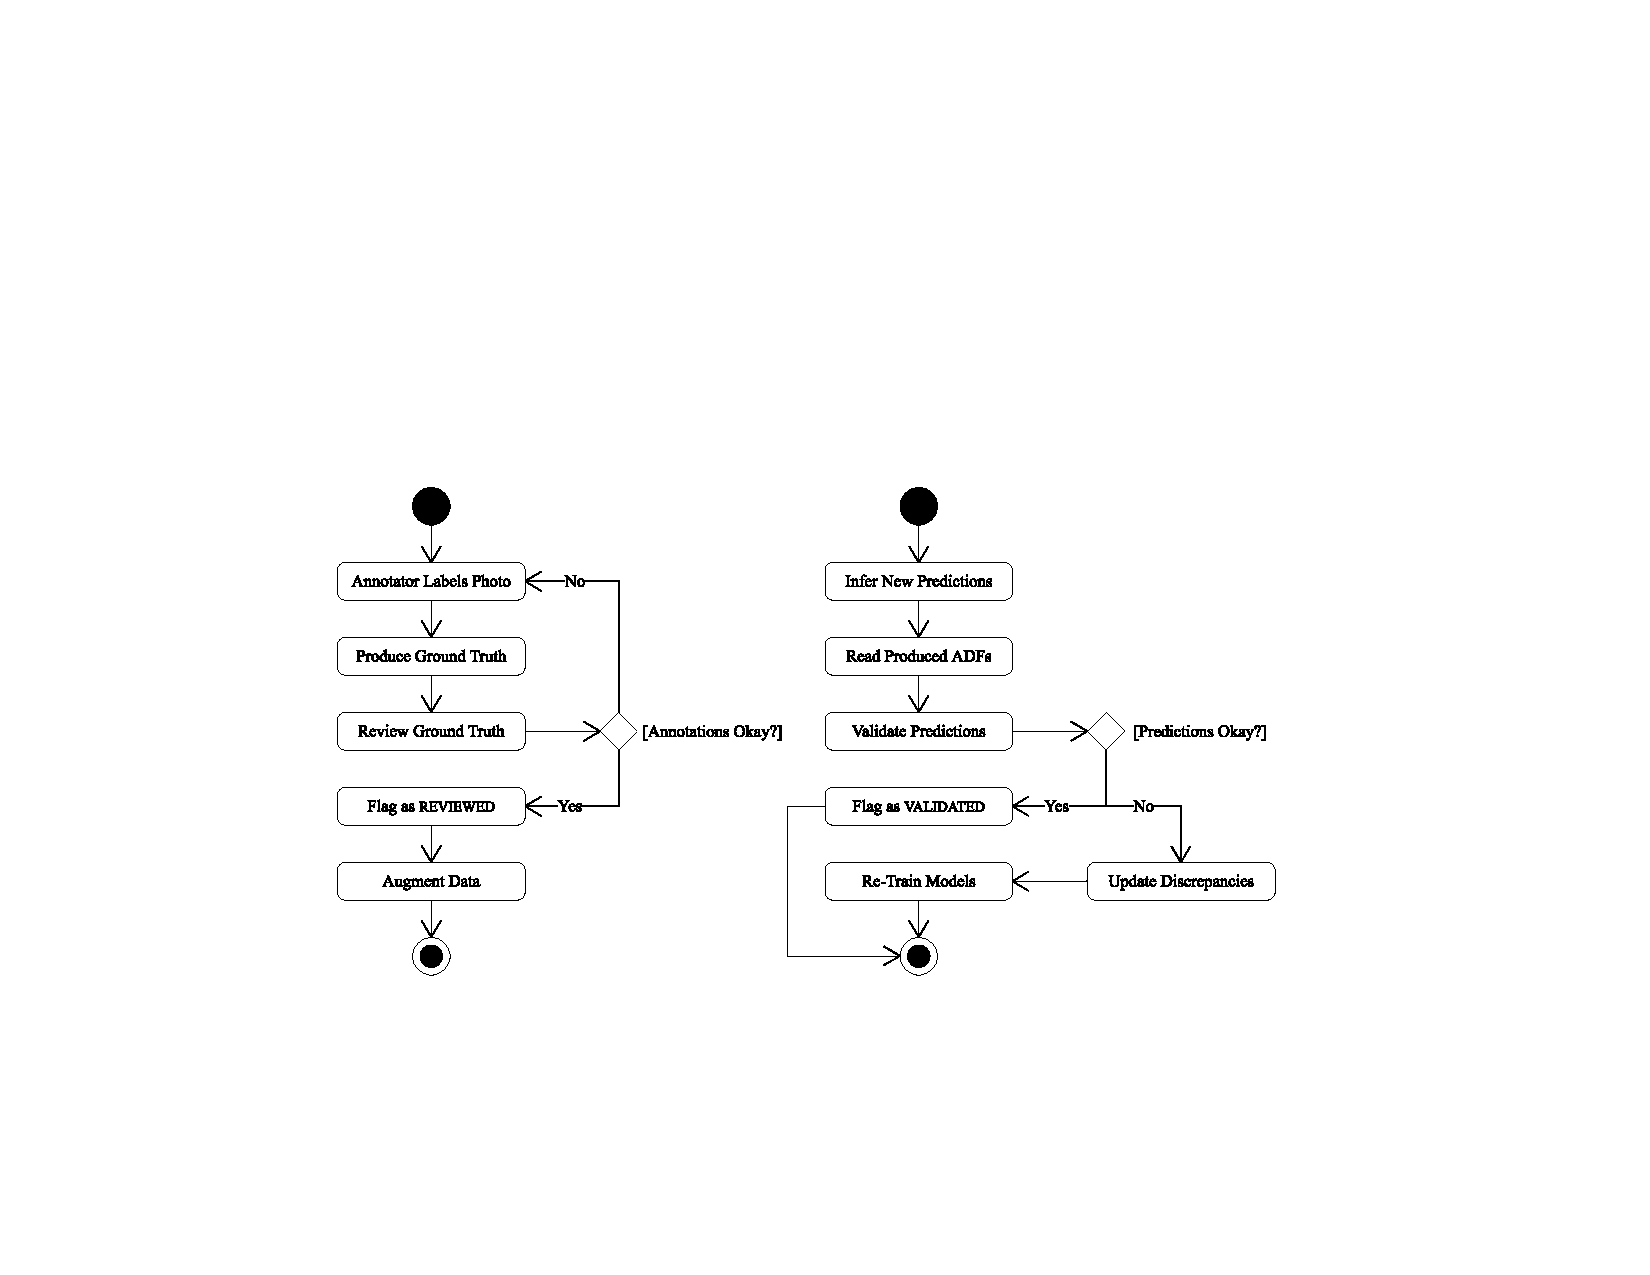
\includegraphics[width=\textwidth]{images/dataset/flagging_statemodel}
  \caption[State diagram to represent flagging]{State diagram of for training data (left) and inference data (right).}
  \label{fig:dataset:postprocessing:state_diagram_flagging}
\end{figure}

Ground truth annotations encompasses the general process that data taggers annotate data. This process is largely the initial data capture that occurs within our dataset, described by the process outlined in \cref{sec:dataset:process}. As mentioned in \cref{sec:dataset:process:load}, once data is annotated, a second parse is done on the annotations by another reviewer to check for any mistakes. Some of our data is also annotated multiple times, and thus multiple \glspl{adf} are produced. A reviewer will check these files and use the best matches to merge the best data together---for instance, in a single photo, if three annotators mark a given runner's \gls{lop} as \textsc{yes} whereas one annotator marks it as \textsc{maybe}, the reviewer may choose to update the \textsc{maybe} to the more likely value.

Once ground truth annotations are inspected for a second time, the annotations in the \gls{adf} file are \textit{flagged} as `\textsc{reviewed}'. We only allow reviewed data to be augmented (\cref{sec:dataset:postprocessing:augmentation}) and thus trained in our \gls{ai} model. This method allows us to maintain a high level of quality and integrity of input data.

The second flag is set on \textit{predicted} \gls{adf} data generated by the \gls{ai}. As the \gls{ai} model produces \gls{adf} files (see \cref{ch:processing_pipeline}), we are able to perform a second parse on the predicted data by loading the predicted \glspl{adf} into Argus' validation mode. Here, a human validates that the predictions made by the model are indeed correct, and if not, we are able to update any discrepancies where needed (via Argus modifications) and feed this corrected invalid data into the model again to correct any mistakes it is making. Here we can flag the predicted data as `\textsc{validated}'. In turn, predications that are validated help ensure that mistakes made by the \gls{ai} model are amended. 

Additional flags that may be considered for future work include `\textsc{creator}', a first class concept that captures the source of who initially created the data, reviewed the data and validated the data. In doing so, quality analysis of annotators can be tracked. Furthermore, a `\textsc{merge}' flag could be considered, whereby the merge of multiple \glspl{adf} on the same source image are made. This would help track when such merges occur and how frequently they occur. We leave such suggestions open for future improvements of Argus.

\begin{landscape}
\begin{figure}[p]
  \centering
  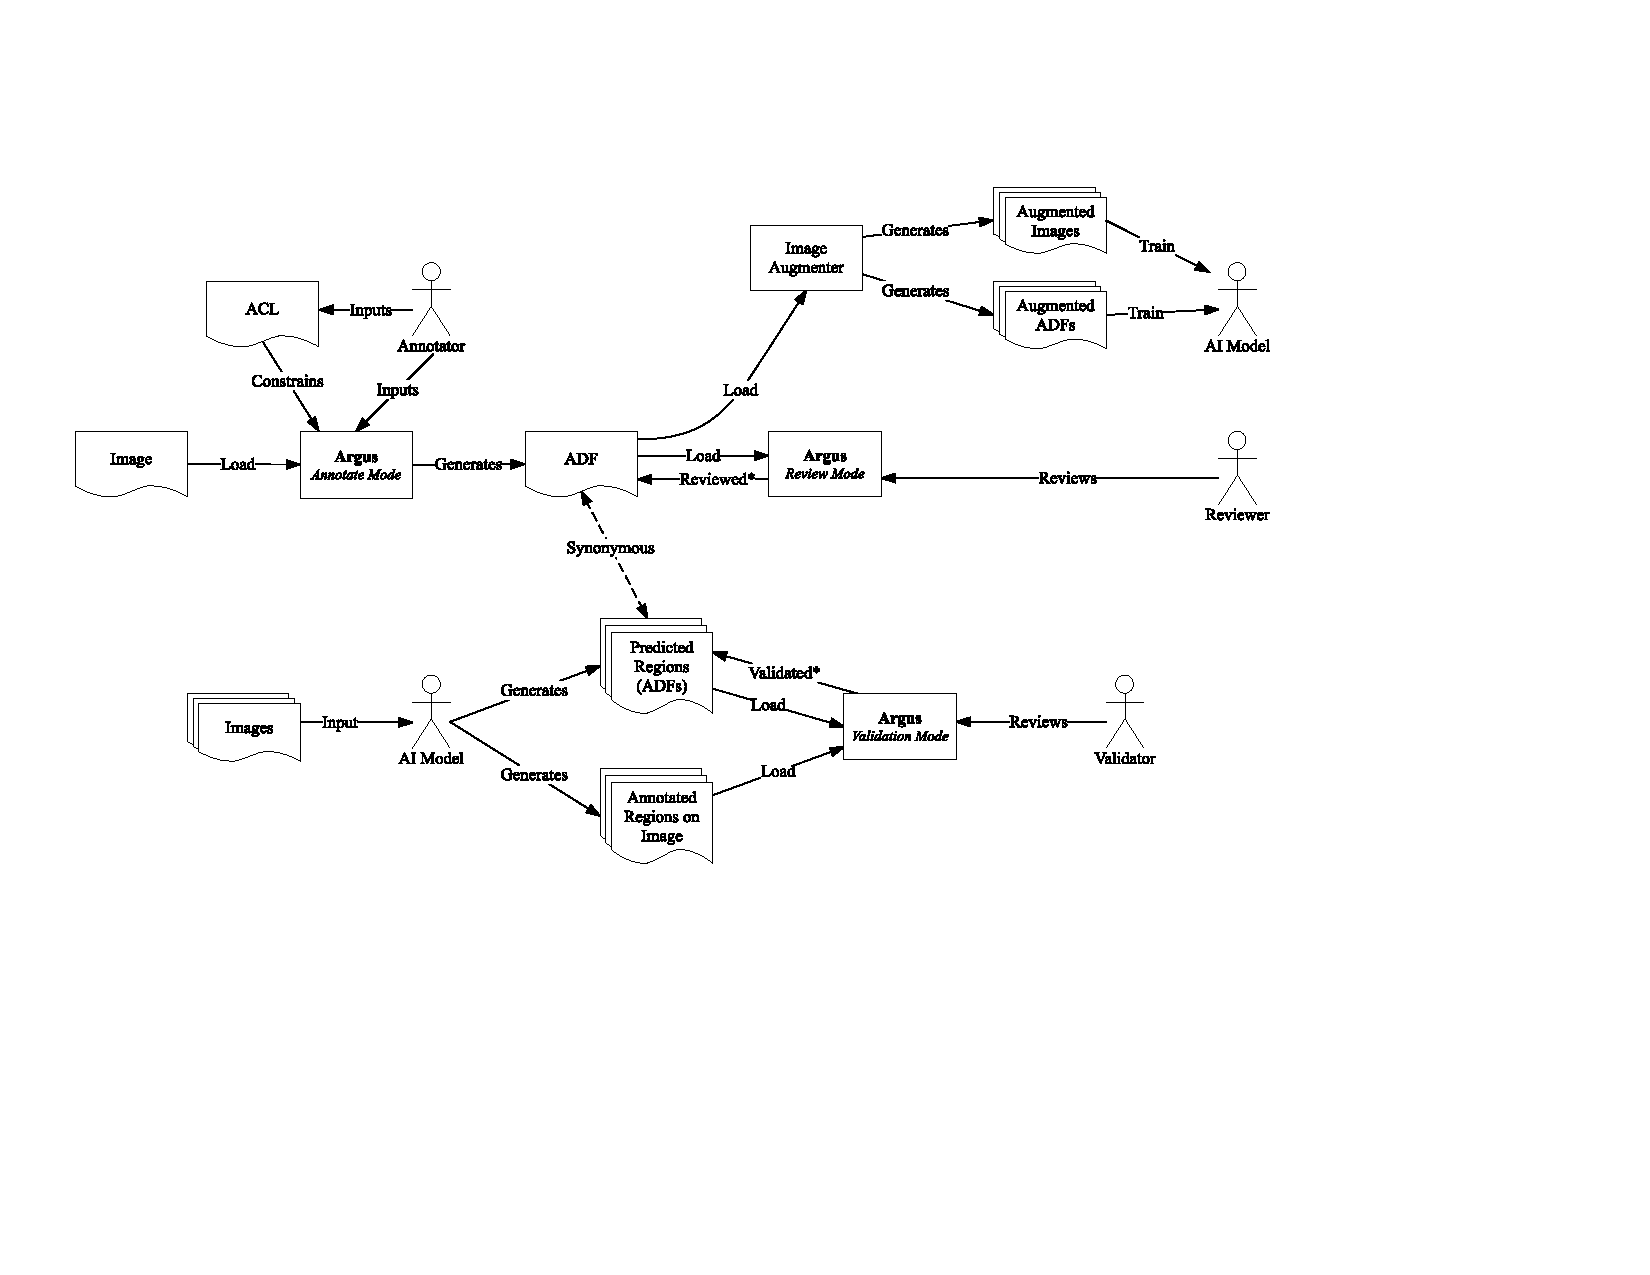
\includegraphics[width=1.1\paperwidth]{images/dataset/overview}
  \caption[Overview of processing made on our dataset]{A general outline of the processing done on the dataset and all relevant actors and associated files. Asterisks indicate where flags have marked annotations as \textsc{reviewed} and predictions as \textsc{validated}.}
  \label{fig:dataset:postprocessing:overal_data_processing}
\end{figure}
\end{landscape}

\subsection{Data Augmentation}
\label{sec:dataset:postprocessing:augmentation}

Previous works show that augmenting data makes a classifier more robust in its detection \citep{Yaeger:1996tq,Baird:1992ih,Wong:2016cv}. A solid augmentation strategy is applied to make the training data for our models more extensive and variable by generating deformations and defects and thereby producing synthetic data. We therefore motivate the need to augment our datasets by producing varied images of the same source image, rapidly fortifying our training data with more images in our dataset.

For our network, we manually tagged 803 images over a total of 14 different marathon events using our concrete Argus implementation (\cref{ch:dataset}) within our dataset. We decided on an augmentation strategy using a 1:50 ratio (thereby to produce a further 40,150 augmented images from these original 803 images). We split the dataset into 90\% for training and 10\% for validation. The specific quantities of images and annotations chosen for training and validation are described in \cref{tab:dataset:postprocessing:augmentation_quantities}. An annotation to image ratio less than 1 indicates there were more crowded photos in the sample set.

\begin{table}[t]
\centering
\caption[Breakdown of training and validation data]{Breakdown of images and annotations (runners) used for training and validation.}
\label{tab:dataset:postprocessing:augmentation_quantities}
  \tablefit{
    \begin{tabular}{@{}l|lll|lll@{}}
    \toprule
    \multirow{2}{*}{\textbf{Image Type}} & \multicolumn{3}{l}{\textbf{Training}}                                 & \multicolumn{3}{l}{\textbf{Validation}}                               \\ \cmidrule(l){2-7} 
                                         & \textbf{Images} & \textbf{Annotations} & \textbf{Annotations / Image} & \textbf{Images} & \textbf{Annotations} & \textbf{Annotations / Image} \\ \midrule
    \textbf{Original}                    & 722             & 850                  & 1.177                        & 81              & 109                  & 1.346                        \\
    \textbf{Augmented}                   & 36100           & 33098                & 0.917                        & 4050            & 4266                 & 1.053                        \\ \midrule
    \textbf{Total}                       & 36822           & 33948                & 0.922                        & 4131            & 4375                 & 1.059                        \\ \bottomrule
    \end{tabular}
  }
\end{table}

Our augmentation strategy consisted of the following:

\begin{enumerate}
  \item perform affine transformations on every image,
  \item distort colour channels by adding intensities of $\pm45\%$ applied 50\% of the time,
  \item distort colour channels by multiplying intensities between a range of $[0.5, 1.5]$ applied 50\% of the time,
  \item apply one of a gaussian, average or median blur 30\% of the time.
\end{enumerate}

Our affine transformations consisted of translations in both the $x$ and $y$ axes shifted between $\pm35\%$, rotated between $\pm45\degree$, and sheared between $\pm5\%$. These transformations were implemented using the \textit{imgaug} library\footnoteurl{https://github.com/aleju/imgaug}{11 August 2017} for Python. See \cref{fig:dataset:postprocessing:augmentation} for examples.

As these transformations occur randomly, there are cases where translation, shearing and rotation occur extremely (e.g., \cref{fig:dataset:postprocessing:augmentation:crop1,fig:dataset:postprocessing:augmentation:crop2}). This causes some bibs to be cropped off the image. Therefore, we remove these from the transformed \gls{adf} file as we cannot have a bounding box referencing outside the image.

\begin{figure}[h!]
  \centering
  \hspace{\fill}
  \begin{subfigure}[b]{0.475\textwidth}
    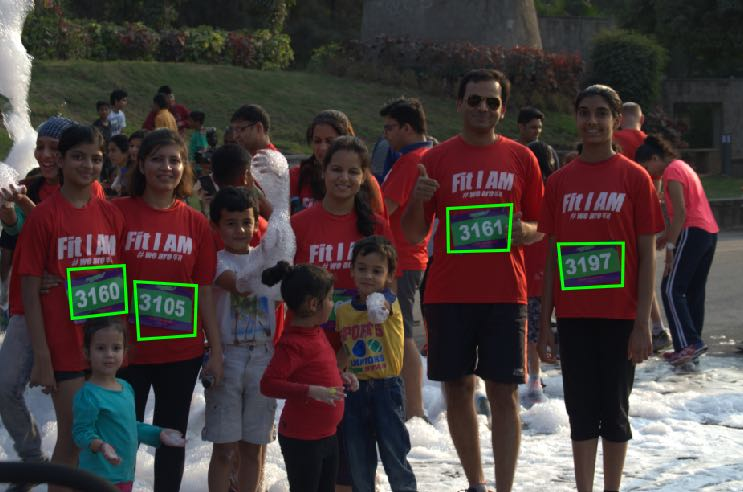
\includegraphics[width=\textwidth]{images/dataset/augmentation/original}
    \caption{Original annotated image.}
  \end{subfigure}
  \hspace{\fill}
  \begin{subfigure}[b]{0.475\textwidth}
    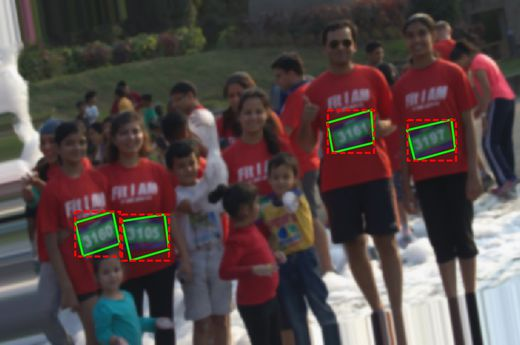
\includegraphics[width=\textwidth]{images/dataset/augmentation/slight_rotate_blur}
    \caption{Slight rotation with blur.}
  \end{subfigure}
  \hspace{\fill}
  \bigskip
  \\
  \hspace{\fill}
  \begin{subfigure}[b]{0.475\textwidth}
    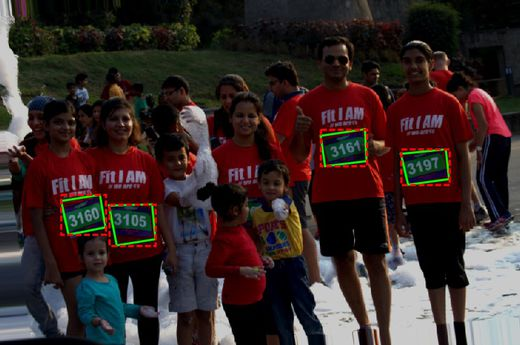
\includegraphics[width=\textwidth]{images/dataset/augmentation/neg_multiply}
    \caption{Darkened channels}
  \end{subfigure}
  \hspace{\fill}
  \begin{subfigure}[b]{0.475\textwidth}
    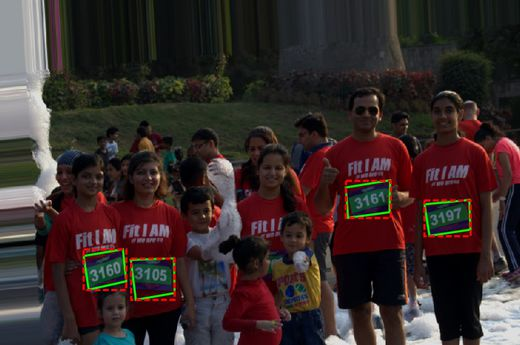
\includegraphics[width=\textwidth]{images/dataset/augmentation/offset}
    \caption{Slight translation.}
  \end{subfigure}
  \hspace{\fill} 
  \bigskip
  \\
  \hspace{\fill}
  \begin{subfigure}[b]{0.475\textwidth}
    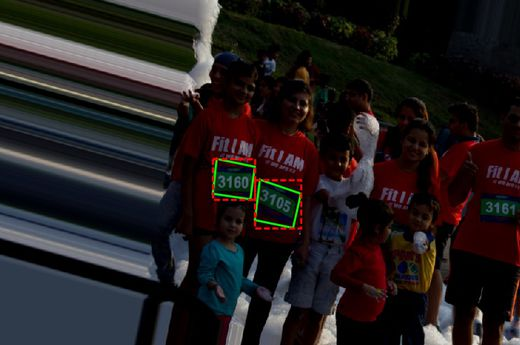
\includegraphics[width=\textwidth]{images/dataset/augmentation/dark}
    \caption{Darkened channels with translation.}
    \label{fig:dataset:postprocessing:augmentation:crop1}
  \end{subfigure}
  \hspace{\fill}
  \begin{subfigure}[b]{0.475\textwidth}
    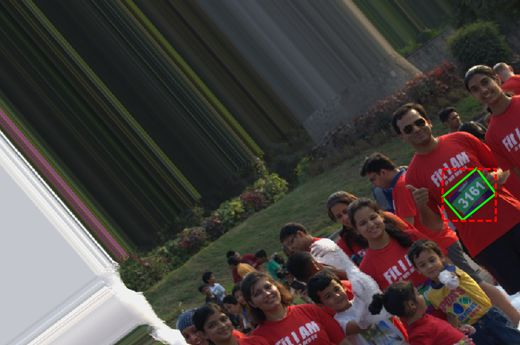
\includegraphics[width=\textwidth]{images/dataset/augmentation/large_offset_rot}
    \caption{Large translation with strong rotation.}
    \label{fig:dataset:postprocessing:augmentation:crop2}
  \end{subfigure}
  \hspace{\fill}
  \bigskip
  \\ 
  \caption[Various augmented images from our dataset]{Various instances of our augmented dataset. Here the \gls{adf} annotation files are drawn directly onto the source image, with the $BibSheet$ polygon shown in green and its respective derived bounding box attribute in red, dotted.}
  \label{fig:dataset:postprocessing:augmentation}
\end{figure}
